\subsection{Countdown-cd4: the central pass@k ranking reversal}
\label{sec:results-countdown}

Countdown-cd4 is the benchmark on which the ranking-reversal claim is sharpest. Diffusion models lead at deterministic and low-$k$ evaluation, but autoregressive models overtake decisively as the sampling budget grows. Figure~\ref{fig:countdown-base} and Table~\ref{tab:countdown-base-passk} are the central empirical evidence for the thesis.

\begin{figure}[!htbp]
\centering
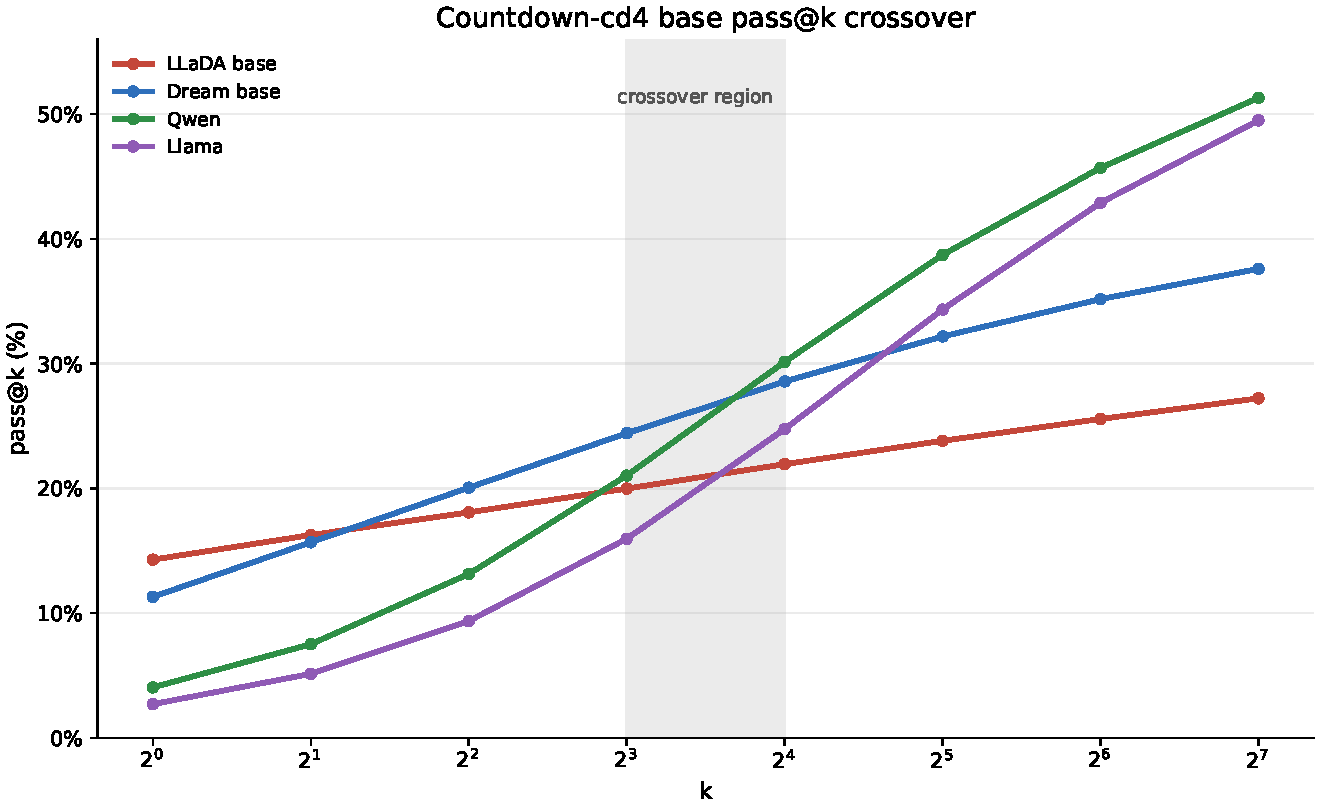
\includegraphics[width=0.92\textwidth]{images/countdown_base_crossover.pdf}
\caption{Countdown-cd4 base pass@k crossover. Diffusion models lead at pass@1; Qwen and Llama overtake by large $k$. The crossover sits near $k=8$--$16$ in this evaluation.}
\label{fig:countdown-base}
\end{figure}

\begin{table}[!htbp]
\centering
\caption{Countdown-cd4 base pass@k, $n=128$, temperature $=0.7$. Diffusion-paradigm ordering at pass@1 reverses to autoregressive-paradigm ordering at pass@128.}
\label{tab:countdown-base-passk}
\scriptsize
\resizebox{\textwidth}{!}{%
\begin{tabular}{lcccccccc}
\toprule
\textbf{Model} & \textbf{1} & \textbf{2} & \textbf{4} & \textbf{8} & \textbf{16} & \textbf{32} & \textbf{64} & \textbf{128} \\
\midrule
LLaDA-Base & 0.143 & 0.163 & 0.181 & 0.200 & 0.219 & 0.238 & 0.256 & 0.272 \\
Dream-Base & 0.113 & 0.157 & 0.201 & 0.244 & 0.286 & 0.322 & 0.352 & 0.376 \\
Qwen-Base  & 0.040 & 0.075 & 0.131 & 0.210 & 0.301 & 0.387 & 0.457 & 0.513 \\
Llama-Base & 0.027 & 0.051 & 0.094 & 0.160 & 0.248 & 0.343 & 0.429 & 0.495 \\
\bottomrule
\end{tabular}}
\end{table}

At pass@1 the ordering is LLaDA-Base $>$ Dream-Base $>$ Qwen-Base $>$ Llama-Base. At pass@128 it becomes Qwen-Base $>$ Llama-Base $>$ Dream-Base $>$ LLaDA-Base. This is not a small fluctuation: Qwen-Base rises from $0.040$ to $0.513$, while LLaDA-Base rises from $0.143$ to only $0.272$. The result supports the concentration-versus-diversity reading developed in Section~\ref{sec:results-diversity} and is the strongest single piece of paradigm-level evidence in the thesis.

The instruct-templated condition is more model-dependent than the base condition. Dream-Instruct retains a useful pass@k profile, Llama-Instruct becomes the strongest high-$k$ model, Qwen-Instruct plateaus early, and LLaDA-Instruct shows a checkpoint-level collapse to pass@128$=0.055$ that does not appear in the same model on GSM8K (pass@1$=0.756$) or Trip Planning (pass@1$=0.010$) and that does not appear in LLaDA-Base on Countdown (pass@1$=0.143$). The instruct-templated row is therefore a property of this specific instruction-tuned checkpoint on this constrained planning task, not a generic dLLM-instruct artifact, and is included for completeness rather than as evidence for the paradigm-level claim.

\begin{table}[!htbp]
\centering
\caption{Countdown-cd4 instruct-templated pass@k, $n=128$, temperature $=0.7$. The LLaDA-Instruct row is a checkpoint-specific collapse and is not used as evidence for the paradigm-level claim.}
\label{tab:countdown-instruct-passk}
\scriptsize
\resizebox{\textwidth}{!}{%
\begin{tabular}{lcccccccc}
\toprule
\textbf{Model} & \textbf{1} & \textbf{2} & \textbf{4} & \textbf{8} & \textbf{16} & \textbf{32} & \textbf{64} & \textbf{128} \\
\midrule
LLaDA-Instruct & 0.024 & 0.028 & 0.032 & 0.036 & 0.041 & 0.047 & 0.052 & 0.055 \\
Dream-Instruct & 0.091 & 0.125 & 0.160 & 0.196 & 0.232 & 0.264 & 0.293 & 0.323 \\
Qwen-Instruct  & 0.078 & 0.107 & 0.134 & 0.159 & 0.181 & 0.199 & 0.213 & 0.221 \\
Llama-Instruct & 0.058 & 0.103 & 0.167 & 0.244 & 0.316 & 0.376 & 0.424 & 0.462 \\
\bottomrule
\end{tabular}}
\end{table}

An earlier smaller Countdown run was used to scope flat-versus-templated prompting before the canonical refreshed run reported above. The diagnostic confirms that Dream-Instruct and Qwen-Instruct shift substantially under flat prompting while LLaDA-Instruct does not, but its absolute scores are not directly comparable to Tables~\ref{tab:countdown-base-passk}--\ref{tab:countdown-instruct-passk} because of differing generation length and evaluation set; the full diagnostic is reproduced in Appendix~\ref{sec:appendix-countdown-prompt}.
